\chapter{Conclusions}

The lofty goal set out at the beginning of this thesis was to develop the architecture of a quantum computer. Unfortunately,
as I hope has become clear throughout the course of your reading, reaching the goal of a universal quantum computer
is not yet within our grasp. However, what I have aimed to do here is to have made progress towards a general purpose quantum machine at each
level of the quantum computing stack, from the high-level architecture in Chapter~\ref{sec:arch}, to the low level
of designing materials for qubits in Chapter~\ref{sec:majoinas}. As I come to the close of this thesis, I will reflect on the outstanding
challenges of realizing a quantum computer, including on areas where I think there is significant risk moving forwards.

\section{Controlling Qubits}
At the top of the stack, in Chapter~\ref{sec:arch}, I discussed the challenges of designing quantum devices that can scale up to a large number of
control and readout lines that a useful quantum machine would require. In addition, I presented architectures that lower the
requirements on both the number of dc and rf lines and on the power dissipation required to control a quantum device. Today, the effort to build
CryoCMOS architectures for controlling qubits has been joined by several companies and groups, including Google~\cite{gcryocmos}, Intel and Delft university~\cite{VANDIJK201990},
who are well and truly in the race to build components for scaleable cryogenic operation of both superconducting and semiconducting qubits. The aims of each
of these efforts are twofold, firstly to bring the footprint of the qubit-classical interface under control, the second being
to tame the rapid growth of power consumed at each part of the stack.

In Sec.~\ref{sec:archdesign}, the requirement for control and readout fidelity was also given alongside the requirements for footprint and power. Pointedly,
these two requirements are not listed with the above, since the reality of the modern quantum physics experiment is that the bulky room temperature readout
and control hardware is largely superior to hardware we build for cryogenic operation. This is not surprising, much of the equipment that is currently used
for readout and control, be it oscilloscopes, network analyzers, vector sources and so forth, trade off power and size for flexibility and performance, which
are unfortunately not what is needed to scale quantum systems. The challenge for each of the architectures listed in Chapter~\ref{sec:arch}, and for those
being developed externally, is to match their classical counterparts with a limited subset of the features available in room temperature hardware.
The challenge for physicists, both theoretical and experimental, is to design the next generation of qubit architectures in such a way that they can be easily
controlled by cryogenic control hardware which has a limited amount of flexibility. In the medium term, this may mean trading off the best qubit performance
for more uniform qubits, or slowing down qubits to relax stringent timing requirements.

Chapter~\ref{sec:hall} looks at the miniaturization of microwave circulators, touching on the topic of controlling the footprint of the qubit-classical
interface. In particular, in Sec.~\ref{sec:readout}, we discussed the need to isolate qubits from the noise generated by classical readout hardware without
adding additional losses into the circuit, as any loss between the qubit and first stage amplifier contributes directly to the SNR of our readout, as per
Eq.~\ref{eq:r_snr}. For the qubits presented in this thesis (spin qubits and Majorana based topological qubits), the footprint problem is particularly
stark, as readout frequencies of a few hundred \si{\mega\hertz} would require conventional circulators on to order of \SIrange{30}{70}{\centi\meter}.
Utilizing the slow-traveling edge-magnetoplasmons (EMPs) in the quantum (anomalous) Hall effect, circulators with a size of order a few hundred \si{\micro\meter}
were realized. While isolation of \SI{25}{\decibel} was achieved, the insertion loss of this first generation of circulators was not sufficient to
be generally useful in qubit experiments. The source of this loss is caused largely by the impedance mismatch between the EMP ($\sim \SI{25}{\kilo\ohm}$) and the
\SI{50}{\ohm} transmission line.

Understanding the source of this insertion loss, however, gives us several solutions towards improving these systems. One obvious, though perhaps
not useful solution is to operate at higher filling factors, where multiple parallel paths lead to a reduction in the impedance of the edge, as
given by Eq.~\ref{eq:hallsigma}. This solution would require either a larger Hall droplet or operation at higher frequencies, nor would this solution
be possible for samples using the quantum anomalous Hall effect. Alternatively, as the problem is impedance matching, we can use conventional matching
techniques to improve the insertion loss, for example, the use of an LC matching network. A promising approach given in~\cite{bosco2016self} is to use
an intrinsic matching effect in the edges to achieve self-matching at specific frequencies. Such a device geometry promises perfect transmission at these
frequencies.

\section{Scaleable Qubit Designs}
Designing scalable gate layouts for qubit devices remains an open challenge. In Chapter~\ref{sec:spinqubit} this is exactly the challenge that we aim to
tackle, in two ways. First is the design of a modular layout that allows for a design element to be tiled directly, and is presented in Sec.~\ref{sec:5dot}.
A tiling of this design is shown in Fig.~\ref{fig:scaledes}. For such a technique to be genuinely scalable, several additional technical developments
must be made. The first is reliable dispersive gate sensing, as the use of proximal charge sensors in such a design is infeasible. Here such sensors are marked in green.
There has been significant progress in the field towards the use of such sensors for spin readout, with many demonstrations of single-shot readout using dispersive
gate sensing appearing in the past year~\cite{Nnano_dzurak,PhysRevApplied.11.044061}, albeit with fidelities below what would be necessary for a scalable qubit
device. Further work to investigate sources of noise in dispersive gate sensing will be required to scale the technique. The work presented in Sec.~\ref{sec:pockets}
investigates one such source of noise, however additional work will be necessary to improve the fidelity of gate-based readout techniques.

As gate density is increased, there is an additional difficulty in breaking out the required control lines, as was discussed in Sec~\ref{sec:control}. The need for
couplers that operate over intermediate and long length scales is partially solved by the use of an intermediate quantum state. Since the publication of the initial work in
Sec.~\ref{sec:5dot}, coherent manipulation of spins via the intermediate quantum state has been demonstrated~\cite{s41467-019-09194-x}, validating the concept
and clearing the path towards large-scale devices. Over long length scales, work performed to couple spin to resonators should allow coherent coupling over
\si{\milli\meter}-length-scales. Although preliminary results demonstrating strong coupling to resonators have been published~\cite{nature11559,2019arXiv190500776B},
coherent manipulation of two spins over large length scales has not been shown at the time of publication. In a similar vein, there exists theoretical work suggesting
coupling via quantum Hall edge states~\cite{dohertyqhe}. However, an experimental demonstration of such a technique has not yet been performed.

\begin{figure}
    \includegraphics[width=0.85\linewidth]{scaledes}
    \caption[Scaleable qubit designs]{\label{fig:scaledes} (a) The design for a 5 quantum dot device, as presented in Sec~\ref{sec:5dot}, showing a path towards creating a 1D
    chain of singlet-triplet qubits. (b) A qubit chip with 6 5-dot devices, controlled by a total of 168 control lines. Superconducting resonators are used for fast,
    frequency multiplexed charge and gate-based readout. A total of 32 readout channels are bonded on this device.}
\end{figure}

In Fig.~\ref{fig:scaledes} (b), a chip design is shown with the on-chip routing of a total of 168 control lines. The device presented there contains 6 sets of two-qubit devices,
each of which is coupled by an intermediate quantum state. As devices grow larger, the requirements for on-chip routing of signals becomes more acute, particularly
while wire-bonding is used to interface to the qubit chip. On this device, routing was performed manually with the assistance of the Altium EDA tool, with readout and
fast pulsing lines broken out to the edges of the device, to make the bonding of such a device feasible, and to reduce the stray inductance and capacitance of bond-wires.
A device with the same design was used in Sec.~\ref{sec:gooseberry} to validate the design of the CryoCMOS architecture, demonstrating the feasibility of on-chip routing
for larger devices. Moving forward, the existence of more advanced EDA tools will allow far more of the design process to be automated, which will be crucial as the
number of gates on single devices grows.

Built into the discussion about scaling a quantum computer is the need to error correct noisy qubits. The number of operations per gate that must be performed to correct errors,
as well as the number of physical qubits required to form an error corrected logical qubit is a sensitive function of the qubit error rate and snowballs as the fault-tolerance
threshold if approached~\cite{6657074,nature23460}. The construction of qubits with improved error rates is therefore highly desirable, and may, in fact, be necessary for universal
quantum computation with as few as 1000 logical qubits. To run Shor's algorithm on a 1024-bit number, for example, would require on the order of 50-million physical qubits with
an error rate of $10^{-5}$. The use of topologically protected qubits~\cite{RevModPhys.80.1083}, such as Majorana zero modes~\cite{s41578-018-0003-1}, is the most promising path
to realizing qubits with a significantly improved fidelity; however the materials and techniques challenges, as laid out in Chapter~\ref{sec:majoinas} are formidable.
Nonetheless, continuing advances in the growth of high-quality materials with large spin-orbit interaction, and high-quality superconductivity~\cite{PhysRevLett.119.136803},
and improved designs for scaleable Majorana-based devices~\cite{PhysRevB.95.235305,Plugge} present exciting opportunities for building truly scaleable quantum machines.
Some of these issues are explored in Chapter~\ref{sec:majoinas}, including the design of charge sensors in Sec.~\ref{sec:rfmajo}, and the development of fabrication techniques
in Sec.~\ref{sec:inas_hb}. Moving forward, it is clear that there are some fundamental scientific problems to solve with such devices to prove that they are indeed possible.
Without them, however, it is difficult to see how with current error rates and control schemes, any scaleable quantum machine will be possible.

\section{Closing Remarks}
The field today is focussed on achieving quantum supremacy, that is to run an algorithm on a quantum computer that could not feasibly be
simulated on a classical machine. The consensus at the time of writing is that this will be some variant of Boson sampling~\cite{Aaronson:2011},
performed on approximately 50 qubits~\cite{savage,8322045,10.1038/s41567-018-0131-y}, with companies such as Google, IBM, Rigetti and Ion-Q each having
announced their intention to reach this goal imminently. However, even though IBM announced its 50 qubit processor in November 2017~\cite{ibmq}, Google announced
its Bristlecone chip containing 72 qubits at the March Meeting of the American Physical Society in 2018~\cite{bristlecone,Neill195} and Intel announced
its 49 qubit quantum processor in January at CES 2018~\cite{intelq}, the goal of quantum supremacy lies tantalizingly just out of reach. From a scientific standpoint,
this is perhaps not surprising. There is plenty of evidence that even for the problem of Boson sampling, the quality of qubits must be higher
than expected~\cite{PhysRevX.6.021039,PhysRevLett.117.080501}, the connectivity of qubits must be relatively high~\cite{s41567-018-0124-x},
and that the number of qubits might be larger than thought~\cite{2017arXiv171005867P}.
From the standpoint of a quantum physicist and engineer, this represents an exciting challenge, one that calls for further incremental improvement of qubits,
for new designs that extend the connectivity of qubits and for improved methods of readout and control. From the perspective of the public and the community, however,
there lies some danger, wherein we run the risk of hitting a "Quantum Winter". This would be a period analogous to the "AI Winter"~\cite{crevier1993ai},
a period in the history of artificial intelligence, where persistent hype and an over-selling of the promise of AI, followed by a failure to deliver on these promises,
led to a period of reduced funding and interest in the field. The reason that quantum supremacy has not yet been achieved may not be surprising to those in the
field but has regularly been a source of surprise to members of the public.

\begin{figure}
    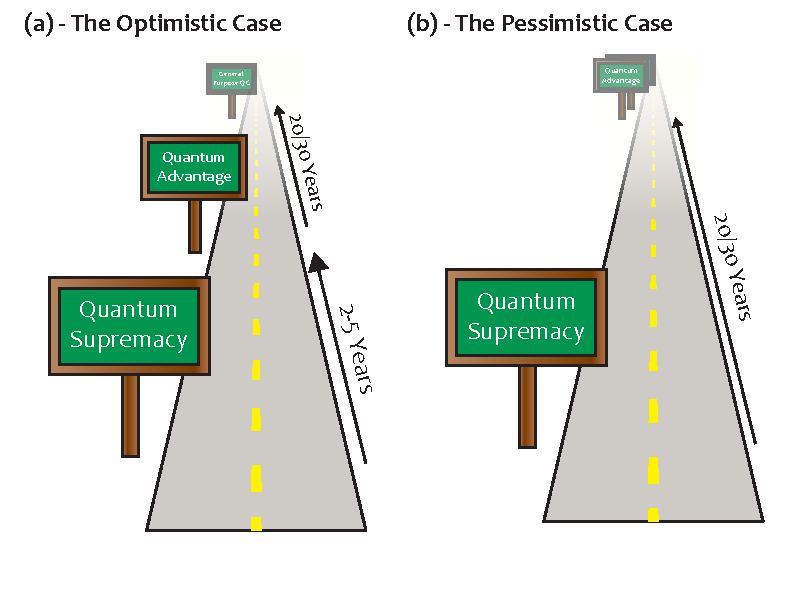
\includegraphics[width=0.7\linewidth]{Roadmap}
    \caption[Roadmap to a quantum computer]{\label{fig:roadmap} The possible paths by which a quantum computer is achieved. (a) In the optimistic case,
    a few years after quantum supremacy is reached, an algorithm demonstrating quantum advantage is achieved, leading to continued interest in the field. (b) In the pessimistic case,
    even though quantum supremacy is reached, the demonstration of an algorithm that shows quantum advantage doesn't occur until a general purpose quantum machine is available.}
\end{figure}

If we assume, however, that we reach the goal of quantum supremacy in the reasonably near future, there are two roadmaps to a general purpose quantum machine, one which
presents great opportunities for quantum computing researchers, the other which presents a risk that we must confront to ensure that development continues sustainably.
These two roadmaps are shown in Fig.~\ref{fig:roadmap}, and relate to the demonstration of quantum advantage, that is the solution of a problem with a quantum computer
that would not have been possible without one. Equivalently, the question is "what is interesting in the NISQ era"~\cite{Preskill2018quantumcomputingin}? In Fig.~\ref{fig:roadmap}
(a), the answer is "something". This may be Variational Quantum Eigensolvers (VQEs)~\cite{nature23879}, it may be some form of machine learning~\cite{PhysRevLett.121.040502},
however there is yet every chance that even these algorithms may turn out to be classically tractable~\cite{Tang:2019:QCA:3313276.3316310,10.1038/nphys3272}, or requires
error correction to the extent that we are pushed to the realm of needing a general purpose quantum machine~\cite{Reiher7555}. In this case, we may live in a world where
Fig.~\ref{fig:roadmap} (b) is true, and there is a long period where a quantum computer is simply a toy. Such a situation would require continued long term investment,
and is not a future that we should ignore in our current push to build a quantum computer.

Despite the risk, it is also true that at no other point in the history of quantum computing has there been such high awareness of the magnitude of the problems
that must be solved. There is constant development in all areas of the stack, from proposals for quantum programming languages to improved equipment for quantum
experiments to even new types of qubits. Together, all of this convinces me that, barring an extraordinary no-go result, a useful quantum computer is not only
achievable but will be realized in the next 20 or so years. I can't predict the form of such a quantum computer, nor how it will be used, however regardless of
its final form, it will confer benefits on all of humanity.
